% --- CHUNK_METADATA_START ---
% needs_review: True
% src_checksum: a387e729f92436e818c56320d986498042b8bbec2b20f59a185ece46c35cdd1c
% --- CHUNK_METADATA_END ---
\chapter{Зведення ендоморфізмів}% --- CHUNK_METADATA_START ---
% needs_review: True
% src_checksum: fbc72cfef8a9e5a11acb9fa09f47f0f56fbddd330f7ca5ebbe328e52998a425d
% --- CHUNK_METADATA_END ---
Під час написання цього розділу я надихався відео з каналу \textit{3blue1brown}, які я вам раджу подивитися, принаймні плейлист щодо лінійної алгебри. Другим джерелом натхнення була книга Джозефа Гріфона \cite{grifone}.% --- CHUNK_METADATA_START ---
% needs_review: True
% src_checksum: 479ce8267a8dc66449e53b838492edeab11f9f116eed87da087547c1cd388ae6
% --- CHUNK_METADATA_END ---
\section{Вступ}% --- CHUNK_METADATA_START ---
% needs_review: True
% src_checksum: b259dc72d8b683f95181cf362a77427e89eb5f523b8d267844312acf75c8bd32
% --- CHUNK_METADATA_END ---
У попередньому розділі ми вивчили поняття ортонормованого базису, корисність якого полягає у спрощенні обчислень координат у базисі та обчисленні проєкції. Це поняття є одним з перших кроків до вивчення SVD\footnote{Singular Value Decomposition}, яке застосовується в багатьох областях, наприклад: зменшення розмірів зображень.
\par
У цьому розділі ми продовжуємо вивчення базисів, щоб зрештою зрозуміти SVD. Ми вивчимо редукцію ендоморфізмів, \textit{to be more precise}, діагоналізацію та тригоналізацію. Для початку: невеличка вправа:% --- CHUNK_METADATA_START ---
% needs_review: True
% src_checksum: c724d8f48a016c11bc237e7ac867213a4de62ac70e8e5b7af983c5583736e72b
% --- CHUNK_METADATA_END ---
\begin{ex}
   Обчислити
   \[
   \begin{bmatrix}
       3 & 1\\
       0 & 2
   \end{bmatrix}^{15} = \underbrace{
       \begin{bmatrix}
       3 & 1\\
       0 & 2
       \end{bmatrix}
       \cdot
       \ldots
       \cdot
       \begin{bmatrix}
       3 & 1\\
       0 & 2
       \end{bmatrix}
   }_{15 \text{ разів}}
   \]
\end{ex}% --- CHUNK_METADATA_START ---
% needs_review: True
% src_checksum: db54f58737d8f17d246be0188ca795e38d99b1523ea21594f4d2a50062df2fef
% --- CHUNK_METADATA_END ---
Це не виглядає дуже легко, чи не так? Наприкінці цього розділу ми знайдемо спосіб спростити обчислення, і в кінці ми розв'яжемо цю вправу.
\par
З лінійної алгебри відомо, що можна представити матрицю відображення в різних базисах, тобто нехай $\{e_i\}$ - базис $E$ і $f$ - відображення. Тоді це відображення в базисі $\{e_i\}$ представлено так:
 \[
A = M(f)_{e_i} = \|f(e_1), \ldots, f(e_n)\|
\] 
Нехай $\{e_i'\}$ - інший базис $E$, тоді ми можемо представити відображення $f$ в цьому базисі також, позначимо: $P = P_{e_i \to e_i'}$ матрицю переходу з базису% --- CHUNK_METADATA_START ---
% needs_review: True
% src_checksum: a455440085569ccfa50055d0bc7764665730f4c664f1b99eaf1ad4cea3c5ff0c
% --- CHUNK_METADATA_END ---
$\{e_i\}$ до бази $\{e_i'\}$
 \[
     A' = M(f)_{e_i'} = P^{-1}AP = \|f(e_1'), \ldots, f(e_n')\|_{e_i'}
\]% --- CHUNK_METADATA_START ---
% needs_review: True
% src_checksum: fc62110b6f4665fe0026522308f37adea92af33580b2a7c7add82761c52f764b
% --- CHUNK_METADATA_END ---
\begin{definition}\label{def:matrice-diagonalisable}
    Матриця $A$ є \textbf{діагоналізованою} якщо існує подібна матриця\footnote{$A$ подібна до $A'$ якщо існує матриця переходу $P$ така що  $A' = P^{-1}AP$}  $A'$ діагональна:
     \[
         A' = 
         \begin{bmatrix} 
         a_{1,1} & 0 & \ldots & 0 \\
         0 & a_{2,2} & \ddots & \vdots\\
         \vdots & \ddots & \ddots & 0\\
         0 & \ldots & 0 & a_{n,n}
        \end{bmatrix} 
    \] 
\end{definition}% --- CHUNK_METADATA_START ---
% needs_review: True
% src_checksum: 63bf784efd9f3eb008441c2a262bd3d1b80786b3b1a31a8757b9c25a4783d594
% --- CHUNK_METADATA_END ---
\begin{definition}
    Матриця $A$ є \textbf{тригоналізованою} якщо існує подібна матриця $A'$ трикутна (верхня/нижня) 
     \[
         A' = 
         \begin{bmatrix} 
         a_{1,1} & a_{1,2} & \ldots & a_{1,n} \\
         0 & a_{2,2} & \ddots & \vdots\\
         \vdots & \ddots & \ddots & a_{n-1,n}\\
         0 & \ldots & 0 & a_{n,n}
        \end{bmatrix} \text{ або } 
         A' = 
         \begin{bmatrix} 
         a_{1,1} & 0 & \ldots & 0 \\
         a_{2, 1} & a_{2,2} & \ddots & \vdots\\
         \vdots & \ddots & \ddots & 0\\
         a_{n, 1} & \ldots & a_{n, n-1} & a_{n,n}
        \end{bmatrix} 
    \] 
\end{definition}% --- CHUNK_METADATA_START ---
% needs_review: True
% src_checksum: 5f36cb427b1a26270fb9aa3171f8dc649052df2172578e9eb24535d8e71fd7cf
% --- CHUNK_METADATA_END ---
Отже, проблеми цієї глави, які ми збираємося вирішити, такі:% --- CHUNK_METADATA_START ---
% needs_review: True
% src_checksum: e36e2423a78b0f5075b2b2706ad1c82fdb9585a3416a6d0dccbc72776563fe3c
% --- CHUNK_METADATA_END ---
\begin{enumerate}
    \item Визначити, чи є ендоморфізм $f$ діагоналізованим/тригоналізованим, тобто чи існує така матриця $A'$.
    \item Визначити матрицю переходу $P$ та матрицю $A'$.
\end{enumerate}% --- CHUNK_METADATA_START ---
% needs_review: True
% src_checksum: 746031095d9367be5953361e604557802b5229ceb1b198f8e1c5eec023f51276
% --- CHUNK_METADATA_END ---
У всьому розділі ми припускаємо, що векторний простір $E$ має скінченну розмірність.% --- CHUNK_METADATA_START ---
% needs_review: True
% src_checksum: f83f4cb55bb9c5b3cbc60c46b58cdb42004864f151f562e6972be1a2ca7cf659
% --- CHUNK_METADATA_END ---
\section{Власні вектори}% --- CHUNK_METADATA_START ---
% needs_review: True
% src_checksum: bfa0ded24a8ac43fd1d9220db52f0511c9dab14b2d78ce78fcafc81151802127
% --- CHUNK_METADATA_END ---
Почнемо з уточнення поняття лінійного відображення та його матриці. Візьмемо для цього матрицю з вправи на початку розділу:
\[
A = \begin{bmatrix} 
       3 & 1\\
       0 & 2
   \end{bmatrix}
\] 
Ця матриця перетворює векторний простір, який ми задаємо, або, спрощуючи, вона перетворює кожен вектор векторного простору. Візьмемо вектор $v_3 = \begin{pmatrix} 1 \\ 1 \end{pmatrix} $, застосовуючи $A$, отримуємо:
 \[
Av_3 = \begin{bmatrix} 
       3 & 1\\
       0 & 2
   \end{bmatrix}\begin{bmatrix} 1 \\ 1 \end{bmatrix} = \begin{bmatrix} 3 \\ 0 \end{bmatrix} + \begin{pmatrix} 1 \\ 2 \end{pmatrix} = \begin{bmatrix} 4 \\ 2 \end{bmatrix} 
\]% --- CHUNK_METADATA_START ---
% needs_review: True
% src_checksum: 53748873e68a45b71c636a03328d19fc757a130cd10577ec5dd38db4946a9bc4
% --- CHUNK_METADATA_END ---
\begin{center}
    
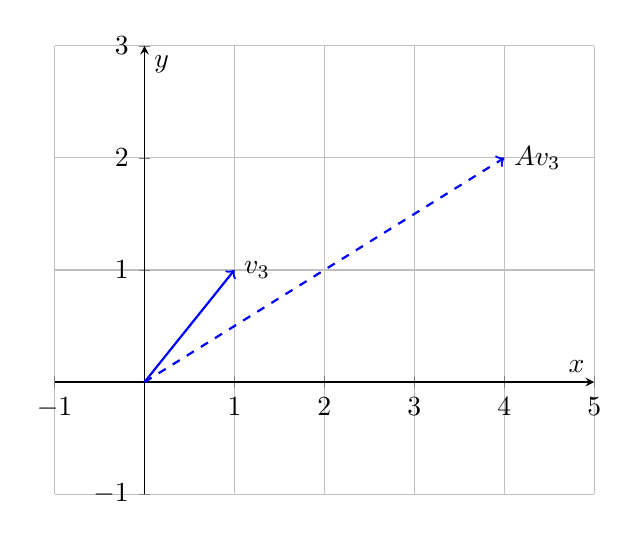
\begin{tikzpicture}
    \begin{axis}[
        axis lines=middle, 
        grid=major, 
        xlabel={$x$}, 
        ylabel={$y$}, 
        ymin=-1, ymax=3,
        xmin=-1, xmax=5
    ]
        % Визначте вихідні вектори
        \addplot[->, thick, blue] coordinates {(0,0) (1,1)};
        \node[right] at (axis cs:1,1) {$v_3$};

        % Визначте трансформовані вектори
        \addplot[->, thick, blue, dashed] coordinates {(0,0) (4,2)};
        \node[right] at (axis cs:4,2) {$A v_3$};
    \end{axis}
\end{tikzpicture}
\end{center}% --- CHUNK_METADATA_START ---
% needs_review: True
% src_checksum: c8eddafdabc468a12a779b174e90bdbbddeb623438e52e27b1a870129d645880
% --- CHUNK_METADATA_END ---
Можна помітити, що вектор $Av_3$ більше не знаходиться на тій самій лінії, що й вектор $v_3$, що логічно, оскільки, якби вектори були на одній лінії після перетворення, це не мало б сенсу.
Однак, іноді трапляються випадки, коли вектор, застосований до матриці, залишається на тій самій лінії, наприклад, вектор $v_2 = \begin{pmatrix} -1 \\ 1 \end{pmatrix} $, де $Av_2 = \begin{pmatrix} -2 \\ 2 \end{pmatrix} = 2v_2 $% --- CHUNK_METADATA_START ---
% needs_review: True
% src_checksum: 3f4b5a2eab7d09a193bb48234f784fd0500a5a1563461a78ec7dc45a4abe55d8
% --- CHUNK_METADATA_END ---
\begin{center}
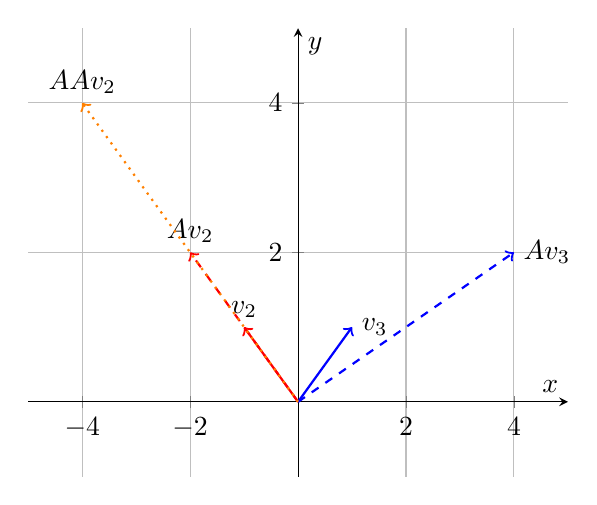
\begin{tikzpicture}
    \begin{axis}[
        axis lines=middle, 
        grid=major, 
        xlabel={$x$}, 
        ylabel={$y$}, 
        ymin=-1, ymax=5,
        xmin=-5, xmax=5
    ]
        % Визначити початкові вектори
        \addplot[->, thick, red] coordinates {(0,0) (-1, 1)};
        \node[above] at (axis cs:-1,1) {$v_2$};
        
        \addplot[->, thick, blue] coordinates {(0,0) (1,1)};
        \node[right] at (axis cs:1,1) {$v_3$};

        % Визначити перетворені вектори
        \addplot[->, thick, red, dashed] coordinates {(0,0) (-2,2)};
        \node[above] at (axis cs:-2,2) {$A v_2$};
        
        \addplot[->, thick, blue, dashed] coordinates {(0,0) (4,2)};
        \node[right] at (axis cs:4,2) {$A v_3$};

        \addplot[->, thick, orange, dotted] coordinates {(0,0) (-4,4)};
        \node[above] at (axis cs:-4,4) {$A A v_2$};
    \end{axis}
\end{tikzpicture}
\end{center}% --- CHUNK_METADATA_START ---
% needs_review: True
% src_checksum: f0865ddb0d189a62787148c9921474158e89812893ff7f5306eec98881902765
% --- CHUNK_METADATA_END ---
І це не лише випадок вектора $\begin{pmatrix} -1 \\ 1 \end{pmatrix} $, якщо взяти будь-який вектор, породжений $v = \begin{pmatrix} -1 \\ 1 \end{pmatrix} $, ми отримаємо $Av = 2v$.
Такі вектори $v$ та скаляри (тут: 2) називаються власними векторами та власними значеннями відповідно. Отже, маємо формальне визначення:% --- CHUNK_METADATA_START ---
% needs_review: True
% src_checksum: 6f65d300d8dcb289daa1913b1f3036a9ac4df8dce62a7501a703b883c85b7e50
% --- CHUNK_METADATA_END ---
\begin{definition}
    Нехай $f$ — ендоморфізм у $E$, а вектор $v \in E$ називається \textbf{власним вектором} для $f$, якщо:
     \begin{enumerate}
        \item $v \neq 0$
        \item Існує дійсне число $\lambda$ таке, що  $f(v) = \lambda v$
    \end{enumerate}
    Скаляр $\lambda \in \R$ називається \textbf{власним значенням} що відповідає $v$.
\end{definition}% --- CHUNK_METADATA_START ---
% needs_review: True
% src_checksum: 8d6f015d17f0abf73d562b2fcade1f9ce8da6e829052fe852d27a804164c13f9
% --- CHUNK_METADATA_END ---
\begin{intuition}
   Власні вектори — це вектори, які під дією $f$ не змінюють напрямків, лише довжину (і навіть не завжди). Це спрощує обчислення таких векторів. Чи можете ви обчислити $A^3v_3$? Не дуже легко, а вектор $A^3v_2$? 
   \[
    Av_2 = 2v_2 \implies A^2v_2 = 2\cdot 2v_2 = 4v_2 \implies A^3v_2 = 2 \cdot 4v_2 = 8v_2 = \begin{pmatrix} -8 \\ 8 \end{pmatrix} 
   \] 
   Це круто, чи не так?
\end{intuition}% --- CHUNK_METADATA_START ---
% needs_review: True
% src_checksum: e95160f028b2d95e35269b03fdbba6365717d280a82da361b410a33d65ab24ef
% --- CHUNK_METADATA_END ---
З іншого боку, це не єдина корисність власних векторів, і ми повернемося до цього, щоб обговорити це, але спочатку, як знайти такі вектори?% --- CHUNK_METADATA_START ---
% needs_review: True
% src_checksum: 24239d1f10bd0d5f05ad63e362795198d22e9c836bde4895ebccdf0135afeb91
% --- CHUNK_METADATA_END ---
\section{Пошук власних значень}% --- CHUNK_METADATA_START ---
% needs_review: True
% src_checksum: 13b0ede61dd64f7dedbca98bbba8400c2c415f0476dbc974f4b86a03654e9e26
% --- CHUNK_METADATA_END ---
Ми шукаємо вектори, які під дією ендоморфізму $f$ масштабуються на коефіцієнт $\lambda \in \R$, отже, ми повинні розв'язати це рівняння:% --- CHUNK_METADATA_START ---
% needs_review: True
% src_checksum: 033cd21f2fe1093d7a3b35c11741aa3150ad95a605391060449ea0add1cc2e90
% --- CHUNK_METADATA_END ---
\begin{align*}
    && f(v) &= \lambda v\\
    \iff&& Av &= \lambda v \quad \text{ у матричній нотації}\\
    \iff&& Av &= \lambda (Iv) \quad \text{ де } I \text{ є одиничною матрицею}\\
    \iff&& Av - \lambda Iv &= 0\\
    \iff&& (A - \lambda I)v &= 0
\end{align*}% --- CHUNK_METADATA_START ---
% needs_review: True
% src_checksum: 54fc59c3379c369321a8bd4b11a191dd4e09d3fcc1eeb5bc3ce1eee9d2c9dca2
% --- CHUNK_METADATA_END ---
Отже, ми повинні вивчити застосування $(A - \lambda I)$ і пов'язати його з поняттям детермінантів. Нагадаємо: якщо детермінант матриці не дорівнює нулю, то ця матриця (тобто ендоморфізм) є ін'єктивною. У нашому випадку, якщо  $\det(A - \lambda I)$ був би нулем, єдиним вектором  $v$, який давав би  $(A - \lambda I)v = 0$, був би нульовий вектор  $v = 0$, оскільки  $(A - \lambda I)$ є лінійним і (як ми припустили) ін'єктивним. 
\par
З іншого боку, згідно з визначенням, власні вектори не є нульовими, тому ін'єктивний випадок не підходить, отже, щоб мати власні вектори, застосування $(A - \lambda I)$% --- CHUNK_METADATA_START ---
% needs_review: True
% src_checksum: c0eb7dd1aa99ead5c9d932030eaf0651f2dbb1350d1b3b113959c2f476f3c2dd
% --- CHUNK_METADATA_END ---
має бути неін'єктивним, що еквівалентно твердженню, що $\det(A - \lambda I) = 0$. Отже, ми повинні обчислити наступний детермінант:
\[
\det(A - \lambda I) = \det \left(\begin{bmatrix} 
    a_{1,1} & a_{1, 2} & \ldots & a_{1, n}\\
    a_{2,1} & a_{2, 2} & \ldots & a_{2, n}\\
    \ldots & \ldots & \ldots & \ldots\\
    a_{n,1} & a_{n,2} & \ldots & a_{n,n}
    \end{bmatrix}  - 
    \begin{bmatrix} 
        \lambda & 0 & \ldots & 0 \\
        0 & \lambda & \ldots & 0 \\
        \ldots & \ldots & \ldots & \ldots\\
        0 & 0 & \ldots & \lambda
    \end{bmatrix}\right) = 
    \begin{vmatrix} 
    a_{1,1} - \lambda & a_{1, 2} & \ldots & a_{1, n}\\
    a_{2,1} & a_{2, 2} - \lambda & \ldots & a_{2, n}\\
    \ldots & \ldots & \ldots & \ldots\\
    a_{n,1} & a_{n,2} & \ldots & a_{n,n} - \lambda
    \end{vmatrix}
\]% --- CHUNK_METADATA_START ---
% needs_review: True
% src_checksum: 202d0d779c7fd9d48fcaf7cbee2aaf0d018bbf151af905d06eb3a68c0c7a2a52
% --- CHUNK_METADATA_END ---
Розкладаючи цей визначник, ми отримуємо рівняння такого типу:
\[
    (-1)^n\lambda^n + a_{n-1}\lambda^{n-1} + \ldots + a_1\lambda + a_0 = 0
\] 
коренями якого є власні значення $f$ (нагадуємо: власне значення є множником $\lambda$).
Не зосереджуйтеся надто сильно на цьому рівнянні зараз, ми ще до нього повернемося.% --- CHUNK_METADATA_START ---
% needs_review: True
% src_checksum: bf5ce8533f46a4f7d3bb2ec19a9531b9c7c84da26177bfd05b62e7f049ee1840
% --- CHUNK_METADATA_END ---
\begin{prop}\label{prop:polynome-caracteristique}
   Нехай $f$ — ендоморфізм у скінченновимірному векторному просторі $E$ розмірності $n$, а $A$ — матриця, що представляє $f$ у базисі $E$. Власні значення $f$ є коренями полінома:
   \[
   P_f(\lambda) = \det(A - \lambda I)
   \] 
   Цей поліном називається \textbf{характеристичним поліномом} $f$.
\end{prop}% --- CHUNK_METADATA_START ---
% needs_review: True
% src_checksum: 14fc75ccd809e480d739d2a472754a41d41f69e99004bb24fa4505811a704a06
% --- CHUNK_METADATA_END ---
\begin{definition}
    Множина власних значень $f$ називається \textbf{спектром} $f$ і позначається $\operatorname{Sp}_K(f)$ або $\operatorname{Sp}_K(A)$, якщо $A$ — матриця $f$.
\end{definition}% --- CHUNK_METADATA_START ---
% needs_review: True
% src_checksum: e2c4c99332b07d283c4805a8d6067b3a6eb0885afdafc105915cb259b9b4c138
% --- CHUNK_METADATA_END ---
Для уточнення:% --- CHUNK_METADATA_START ---
% needs_review: True
% src_checksum: a5e3776b3752e25e079b4a4ff3afc0162901a7b76024cc083b56bfa4e2c66933
% --- CHUNK_METADATA_END ---
\begin{eg}
   Нехай $f$ ендоморфізм в $\R^2$ матриця представлення якого в канонічному базисі є:
   \[
       \begin{bmatrix} 3 & 1\\ 0 & 2 \end{bmatrix} 
   \] 
   Обчислимо його власні значення:
   \begin{align*}
       && \begin{bmatrix} 3 & 1\\ 0 & 2 \end{bmatrix} v &= \lambda v \\
       \iff && \begin{bmatrix} 3 & 1\\ 0 & 2 \end{bmatrix} v - \lambda I v &= 0\\
       \iff && \left(\begin{bmatrix} 3 & 1\\ 0 & 2 \end{bmatrix}  - \lambda I\right)v  &= 0\\
       \implies && \det \left( \begin{bmatrix} 3 & 1\\ 0 & 2 \end{bmatrix}  - \lambda I \right) &= 0\\
       \implies && \det \left( \begin{bmatrix} 3 & 1\\ 0 & 2 \end{bmatrix}  - \lambda \begin{bmatrix} \lambda & 0\\ 0 & \lambda \end{bmatrix}  \right) &= 0\\
       \implies && \det \left( \begin{bmatrix} 3 - \lambda & 1\\ 0 & 2 - \lambda \end{bmatrix}\right) &= 0\\
                && &= (3-\lambda)(2 - \lambda) = 0
   \end{align*}
   Добре видно, що розв'язки: $\lambda_1 = 3$ та $\lambda_2 = 2$
\end{eg}% --- CHUNK_METADATA_START ---
% needs_review: True
% src_checksum: 745ff8ce1da376f0eac0417d1b613c9bbfdc10a8ac9a92ce5fcf0d22e6c24b88
% --- CHUNK_METADATA_END ---
Тим не менш, можна знайти власні значення, а ми шукали власні \underline{вектори}. І ми тут:% --- CHUNK_METADATA_START ---
% needs_review: True
% src_checksum: 76807a4d62a1c1b3f9131c858a7a8e3b4b1c2dd912ab98cfc70831c74c455316
% --- CHUNK_METADATA_END ---
\section{Пошук власних векторів}% --- CHUNK_METADATA_START ---
% needs_review: True
% src_checksum: b1c16951b8606492536c7b6091686d6ae8882a62f54da1d178856d27e1a5b621
% --- CHUNK_METADATA_END ---
Припустимо, для $q \in \N^{*}$ ми вже знайшли $q$ власних значень матриці $\{ \lambda_1, \ldots, \lambda_q \}$, щоб знайти власні вектори, нам залишається знайти базу для:
\[
    \ker(A - \lambda_iI) \quad \forall i \in \{1, \ldots, q\}
\] 
що еквівалентно:
\[
\left( A - \lambda_i I \right)v = 0 \quad \forall i \in \{1, \ldots, q\}
\]% --- CHUNK_METADATA_START ---
% needs_review: True
% src_checksum: be6b8287736d668df8afe873cfc7115ccfab543d54d6dba9446182b22675f15e
% --- CHUNK_METADATA_END ---
\begin{eg}
   Ще раз матриця  
   \[
       A = \begin{bmatrix} 3 & 1\\ 0 & 2 \end{bmatrix} 
   \] 
   в канонічному базисі $\R^2$. Ми вже знайшли її власні вектори: $\lambda_1 = 3$ та $\lambda_2 = 2$. Тоді, шукаємо вектори:
   \[
       \begin{bmatrix} 3 - \lambda_1 & 1 \\ 0 & 2 - \lambda_1 \end{bmatrix}\begin{bmatrix} x \\ y \end{bmatrix} = \begin{bmatrix} 3 - 3 & 1 \\ 0 & 2 - 3 \end{bmatrix}\begin{bmatrix} x \\ y \end{bmatrix} = \begin{bmatrix} 0 & 1 \\ 0 & -1 \end{bmatrix}\begin{bmatrix} x \\ y \end{bmatrix} = 0 
       \implies \begin{cases}
           y = 0\\
           -y = 0\\
           x \in \R
       \end{cases}
   \] 
   Отже $\ker(A - 3I) = \begin{pmatrix} x \\ 0 \end{pmatrix} =  \operatorname{Vect}(\begin{pmatrix} 1 \\ 0 \end{pmatrix} )$. Ось, наш перший власний вектор: $\begin{pmatrix} 1 \\ 0 \end{pmatrix} $. Для другого:
   \[
       \begin{bmatrix} 3 - \lambda_2 & 1 \\ 0 & 2 - \lambda_2 \end{bmatrix}\begin{bmatrix} x \\ y \end{bmatrix} = \begin{bmatrix} 3 - 2 & 1 \\ 0 & 2 - 2 \end{bmatrix}\begin{bmatrix} x \\ y \end{bmatrix} = \begin{bmatrix} 1 & 1 \\ 0 & 0 \end{bmatrix}\begin{bmatrix} x \\ y \end{bmatrix} = 0 
       \implies \begin{cases}
           x + y = 0
       \end{cases} \implies \begin{cases}
           x = -y
       \end{cases}
   \] 
   Отже $\ker(A - 2I) = \begin{pmatrix} -y \\ y \end{pmatrix} = y \begin{pmatrix} -1 \\ 1 \end{pmatrix} = \operatorname{Vect}(\begin{pmatrix} -1 \\ 1 \end{pmatrix} )  $ і ось другий власний вектор: $\begin{pmatrix} -1 \\ 1 \end{pmatrix} $ (це був наш вектор $v_2$ на початку розділу).
\end{eg}% --- CHUNK_METADATA_START ---
% needs_review: True
% src_checksum: bfe0ade345d9629ebf9cee9294d50062797294071d549c1785fda381e4a6a15c
% --- CHUNK_METADATA_END ---
Нарешті, корисна властивість:% --- CHUNK_METADATA_START ---
% needs_review: True
% src_checksum: b5fe3fa2658dff19e7f53c909d80fba3b08b1479a790a2ef5ddc64002859fde1
% --- CHUNK_METADATA_END ---
\begin{prop}
    Нехай $A \in \mathcal{M}_n(\R)$ з його власними векторами: $\{\lambda_1, \ldots, \lambda_n\}$, тоді:
    \begin{align*}
        &\operatorname{Tr}(A) = \lambda_1 + \ldots + \lambda_n\\
        &\operatorname{det}(A) = \lambda_1 \cdot  \ldots \cdot  \lambda_n\\
    \end{align*}
\end{prop}% --- CHUNK_METADATA_START ---
% needs_review: True
% src_checksum: f6522280fbb2a49df36ea182e9cf15e7e5fa21c740e2767f1cb2a283d07f801e
% --- CHUNK_METADATA_END ---
\section{Діагоналізовані ендоморфізми}% --- CHUNK_METADATA_START ---
% needs_review: True
% src_checksum: 42e680abdbc7cf96f41b775cb88850a76fad72acd49f5231124812d3dff1aa63
% --- CHUNK_METADATA_END ---
Повернімося до корисності власних векторів. Нехай $f$ — ендоморфізм $E$, базою якого є $\{e_1, \ldots, e_n\}$, і $\operatorname{Mat}_{e_i}(f) = A$ — матриця $f$ у цій базі. Розглянемо наступний приклад:% --- CHUNK_METADATA_START ---
% needs_review: True
% src_checksum: b1bcb0822f0c84465899d760c678f05039f6a3f2d3cddb2242be844e1f59462f
% --- CHUNK_METADATA_END ---
\begin{eg}
     Маємо: $A = \begin{bmatrix} 3 & 1\\ 0 & 2 \end{bmatrix} $ у канонічному базисі $e_1 = \begin{bmatrix} 1 \\ 0 \end{bmatrix} $ та $e_2 = \begin{bmatrix} 0 \\ 1 \end{bmatrix} $. Нагадаємо, що ми знайшли два власні вектори:
     \[
     \begin{cases}
         v_1 = \begin{pmatrix} 1 \\ 0 \end{pmatrix} \\
         v_2 = \begin{pmatrix} -1 \\ 1 \end{pmatrix} 
     \end{cases}
     \] 
     Зауважимо, що ці два вектори є лінійно незалежними і, отже, утворюють базис для $\R^2$. Спробуємо змінити базис для $A$, маючи два способи:
      \begin{enumerate}
          \item Можна обчислити координати $f(v_1)$ та $f(v_2)$ у базисі $\{v_1, v_2\}$, маємо:
              \begin{align*}
                  &f(v_1) = 3v_1 = 3 \cdot v_1 + 0 \cdot v_2\\
                  &f(v_2) = 2v_2 = 0 \cdot v_1 + 2 \cdot v_2
              \end{align*}
              І тоді $\operatorname{Mat}_{v_i}(f) = \|f(v_1), f(v_2)\|_{v_i} = \begin{bmatrix} 3 & 0 \\ 0 & 2 \end{bmatrix} $ 
          \item Можна обчислити матрицю $P = P_{e_i \to v_i}$ переходу від базису $\{e_i\}$ до базису $\{v_i\}$ та вивести з неї матрицю $f$ у новому базисі. Маємо:
             \[
            \begin{cases}
                v_1 = \begin{pmatrix} 1 \\ 0 \end{pmatrix} = 1 \cdot e_1 + 0 \cdot e_2 = \begin{pmatrix} 1 \\ 0 \end{pmatrix}_{e_i} \\
                v_2 = \begin{pmatrix} -1 \\ 1 \end{pmatrix} = -1 \cdot e_1 + 1 \cdot e_2 = \begin{pmatrix} -1 \\ 1 \end{pmatrix}_{e_i} \\
            \end{cases}
            \] 
              отже $P = \begin{bmatrix} 1 & -1\\ 0 & 1 \end{bmatrix} $ та $P^{-1} = \begin{bmatrix} 1 & 1 \\ 0 & 1  \end{bmatrix}$ (ви можете перевірити обчислення). І отже:
              \[
                  A' = P^{-1}AP = \begin{bmatrix} 1 & 1 \\ 0 & 1 \end{bmatrix} \begin{bmatrix} 3 & 1 \\ 0 & 2 \end{bmatrix} \begin{bmatrix} 1 & -1 \\ 0 & 1 \end{bmatrix} = \begin{bmatrix} 1 & 1 \\ 0 & 1 \end{bmatrix} \underbrace{\begin{bmatrix} 3 & -2 \\ 0 & 2 \end{bmatrix}}_{AP} = \begin{bmatrix} 3 & 0 \\ 0 & 2 \end{bmatrix} 
              \] 
     \end{enumerate}
     І ось, магія, ми знайшли діагональну матрицю.
\end{eg}% --- CHUNK_METADATA_START ---
% needs_review: True
% src_checksum: 413a1dfd9cd7cd1f178a02fdc7f63469147614941ffcd0311ca8af286d1f8dcf
% --- CHUNK_METADATA_END ---
Далі, узагальнимо те, що ми зробили.% --- CHUNK_METADATA_START ---
% needs_review: True
% src_checksum: 77f963d6a51d6406e8e2c398719648118c2decfe33539ffdaf2d6a2a1de08891
% --- CHUNK_METADATA_END ---
\begin{definition}
    Нехай $\lambda \in K$, позначимо:
    \[
        E_{\lambda} := \{v \in E \mid f(v) = \lambda v \}
    \] 
    $E_{\lambda}$ є векторним простором $E$, який називається \textbf{власним простором}, що відповідає $\lambda$.
\end{definition}% --- CHUNK_METADATA_START ---
% needs_review: True
% src_checksum: d6263778d0675b5987e98c8bc733dec041940c50bf52f18c63986fecfbfdc82e
% --- CHUNK_METADATA_END ---
\begin{remark}
   \begin{enumerate}
       \item Якщо $\lambda$ не є власним значенням $f$, тому $E_\lambda = \{0\}$
       \item Якщо $\lambda$ є власним значенням, тоді:
            \[
                E_\lambda = \{ \text{ власні вектори, асоційовані з } \lambda \} \cup \{0\} \text{ та } \dim E_\lambda \ge 1
           \] 
   \end{enumerate} 
\end{remark}% --- CHUNK_METADATA_START ---
% needs_review: True
% src_checksum: 1267f7e54da5fa5982e2c20354feb1ab54afc84f52353ec7f02a698172136c65
% --- CHUNK_METADATA_END ---
\begin{prop}
    Нехай $\lambda_1, \ldots, \lambda_p$ — попарно різні скаляри. Тоді власні простори $E_{\lambda_1}, \ldots, E_{\lambda_p}$ знаходяться в прямій сумі. Інакше кажучи, якщо $\mathcal{B}_1, \ldots, \mathcal{B}_p$ є базисами $E_{\lambda_1}, \ldots, E_{\lambda_p}$, то сім'я $\{\mathcal{B}_1, \ldots, \mathcal{B}_p\}$ є лінійно незалежною (але не обов'язково породжуючою $E$).
\end{prop}% --- CHUNK_METADATA_START ---
% needs_review: True
% src_checksum: 1379cacc5519b4b0ccc3363240525bcd6703b7b0c2152f3c192d1ac8fdc9fa6f
% --- CHUNK_METADATA_END ---
\begin{preuve}
Нехай $E_{\lambda_1}, \ldots, E_{\lambda_p}$ — власні підпростори, асоційовані з власними значеннями $\lambda_1, \ldots, \lambda_p$ ендоморфізму $f$ векторного простору E. Ми повинні показати, що ці підпростори знаходяться в прямій сумі, тобто, якщо вектор належить їхньому перетину, то він дорівнює нулю.

Візьмемо елемент v, що належить їхній сумі, тобто, він може бути записаний у формі:
\[
    v = v_1 + v_2 + \cdots + v_p
\] 
де $v_i \in E_{\lambda_i}$ для всіх $i$.

Оскільки кожен $v_i$ є власним вектором для $f$, асоційованим з $\lambda_i$, маємо:
\[
    f(v_i) = \lambda_i v_i.
\] 
Застосуємо f до суми:
\[
    f(v) = f(v_1 + v_2 + \cdots + v_p) = f(v_1) + f(v_2) + \cdots + f(v_p).
\] 
Використовуючи лінійність $f$, це дає:
\[
    f(v) = \lambda_1 v_1 + \lambda_2 v_2 + \cdots + \lambda_p v_p.
\] 
Проте, $v$ також є комбінацією цих самих векторів:
\[
    v = v_1 + v_2 + \cdots + v_p.
\] 
Отже, перегрупувавши:
\[
    (\lambda_1 v_1 + \lambda_2 v_2 + \cdots + \lambda_p v_p) - (v_1 + v_2 + \cdots + v_p) = 0.
\] 
Що дає:
\[
    (\lambda_1 - 1) v_1 + (\lambda_2 - 1) v_2 + \cdots + (\lambda_p - 1) v_p = 0.
\] 
Факторизуємо кожен член:
\[
    (\lambda_1 - \lambda) v_1 + (\lambda_2 - \lambda) v_2 + \cdots + (\lambda_p - \lambda) v_p = 0.
\] 
Проте, $\lambda_i$ вважаються попарно різними. З цього випливає, що коефіцієнти є різними, і що сума дорівнює нулю лише тоді, коли всі $v_i$ дорівнюють нулю (оскільки власні підпростори, як правило, знаходяться в прямій сумі).

Таким чином, $v = 0$, що доводить, що власні підпростори знаходяться в прямій сумі.
\end{preuve}% --- CHUNK_METADATA_START ---
% needs_review: True
% src_checksum: 2eaf9f0db0b14b9cd67463a1299269bf5cfef19d7e30ec2ff8476706b6e08893
% --- CHUNK_METADATA_END ---
Таким чином, власні простори завжди знаходяться в прямій сумі, але не обов'язково дорівнюють $E$:
 \[
     E_{\lambda_1} \oplus \ldots \oplus E_{\lambda_p} \underset{\neq}{\subset} E
\] 
що ми маємо, якщо:
\[
\dim E_{\lambda_1} + \ldots + \dim E_{\lambda_p} < \dim E
\]% --- CHUNK_METADATA_START ---
% needs_review: True
% src_checksum: 8213c21d8868f9e71a42e919a3c73e6db70f4d92487c8f81cd623c0b6a5eff0d
% --- CHUNK_METADATA_END ---
\begin{theorem}
    Нехай $f$ ендоморфізм в $E$ і $\lambda_1, \ldots, \lambda_p$ його власні значення, тоді наступні властивості є еквівалентними:
    \begin{enumerate}
        \item $f$ діагоналізовний
        \item  $E$ є прямою сумою своїх власних просторів:  $E = E_{\lambda_1} \oplus \ldots \oplus E_{\lambda_p}$
        \item $\dim E_{\lambda_1} + \ldots + \dim E_{\lambda_p} = \dim E$
    \end{enumerate}
\end{theorem}% --- CHUNK_METADATA_START ---
% needs_review: True
% src_checksum: d98bab212106c45f88afcaf4c1d1068a8a038b038282eaa596a01f7a0469250c
% --- CHUNK_METADATA_END ---
\begin{corollary}
   Якщо $f$ є ендоморфізмом $E$ з $\dim E = n$ і $f$ має $n$ власних значень, попарно відмінних, то $f$ є діагоналізованим.
\end{corollary}% --- CHUNK_METADATA_START ---
% needs_review: True
% src_checksum: f46b8c1decbba48b916ea07ecb3f46837dfe2133dcdb857ca960b42272dbc0f2
% --- CHUNK_METADATA_END ---
Але, оскільки власні значення є коренями характеристичного многочлена (див. твердження \ref{prop:polynome-caracteristique}), ми маємо:% --- CHUNK_METADATA_START ---
% needs_review: True
% src_checksum: bc4db3e8c9322d2f54b8b8bd3927f1fecffd46924cbdb8fb78a3872daab6190f
% --- CHUNK_METADATA_END ---
\begin{prop}
    Нехай $f$ ендоморфізм у $E$ та $\lambda$ власне значення порядку $\alpha$ (тобто $\alpha$ є коренем $P_f(\lambda)$ порядку $\alpha$, тобто $P_f(\lambda) = (X - \lambda)^{\alpha}Q(X)$). Тоді:
   \[
   \dim E_{\lambda} \le \alpha
   \] 
\end{prop}% --- CHUNK_METADATA_START ---
% needs_review: True
% src_checksum: b41b18de71939fc7ee9fcfc5cfb62fe7bf6f6c45faeef5e2ed2cda68c06cae8e
% --- CHUNK_METADATA_END ---
\begin{theorem}
   Нехай $f$ — ендоморфізм у $E$ з $\dim E = n$. Тоді $f$ є діагоналізованим тоді й лише тоді, якщо: 
   \begin{enumerate}
       \item $P_f(X)$ є \underline{розщеплюваним}, тобто:
            \[
                P_f(X) = (-1)^n (X - \lambda_1)^{\alpha_1} \cdot \ldots \cdot (X - \lambda_p)^{\alpha_p}
           \] 
           ($\lambda_i$ є коренями, отже, власними значеннями) і $\alpha_1 + \ldots + \alpha_p = n$. Тоді, якщо сума кратностей коренів дорівнює розмірності векторного простору.
       \item Розмірності власних просторів є \underline{максимальними}, тобто $\forall i \in \{1, \ldots, p\}$
           \[
                \dim E_{\lambda_i} = \alpha_i 
           \] 
   \end{enumerate}
\end{theorem}% --- CHUNK_METADATA_START ---
% needs_review: True
% src_checksum: 7bc3254dd77d12e21d0ae0012946c65aae0bce227475ec669ba11498aee3c5b9
% --- CHUNK_METADATA_END ---
\begin{intuition}
   Не завжди легко зрозуміти ідею через характеристичні поліноми, тому інший спосіб побачити це:
   \begin{enumerate}
       \item Знаходимо власні значення: $\lambda_1, \ldots, \lambda_p$
       \item Потім знаходимо власні підпростори: $E_{\lambda_i} = \ker(f - \lambda_i I)$
       \item Сумуємо розмірності: $\dim E_{\lambda_1} + \ldots + \dim E_{\lambda_p} =: d$.  
           \begin{itemize}
               \item 
                   Якщо $d = \dim E$ тобто якщо сума розмірностей дорівнює розмірності простору $E$, власні підпростори породжують $E$ і отже $f$ діагоналізовний (бо його матриця може бути записана в базисі цих власних векторів).
              \item В іншому випадку кількості лінійних власних векторів недостатньо, щоб породити $E$.
           \end{itemize}
   \end{enumerate}
\end{intuition}% --- CHUNK_METADATA_START ---
% needs_review: True
% src_checksum: 1326f78543a8c10e8d45246f66d8ec9489c9aa11bac835c81e13778416517593
% --- CHUNK_METADATA_END ---
\section{Застосунки}% --- CHUNK_METADATA_START ---
% needs_review: True
% src_checksum: 72ce285d1fc5fa7b57b2a02000cdc6ccee979c0b081f1d7c85b238677961b2ec
% --- CHUNK_METADATA_END ---
\subsection{Обчислення потужності}% --- CHUNK_METADATA_START ---
% needs_review: True
% src_checksum: 2c47f2e80bba8d2cda5a17a86a58856e60564538d0253b3fe8dc8251d0fd4b85
% --- CHUNK_METADATA_END ---
\label{subsec:calcule-de-la-puissance-diagonalisation}
Отже, ми повернулися туди, звідки почали, я вам нагадаю задачу з початку розділу:% --- CHUNK_METADATA_START ---
% needs_review: True
% src_checksum: 98d215165627962d168babff6b5f20ceda296a8c477f58a015e756cba56d37a5
% --- CHUNK_METADATA_END ---
\begin{ex}
   Обчислити 
   \[
   \begin{bmatrix} 
       3 & 1\\
       0 & 2
   \end{bmatrix}^{15} = \underbrace{
       \begin{bmatrix} 
       3 & 1\\
       0 & 2
       \end{bmatrix}
       \cdot
       \ldots
       \cdot
       \begin{bmatrix} 
       3 & 1\\
       0 & 2
       \end{bmatrix}
   }_{15 \text{ разів}}
   \] 
Нагадаємо, що власні вектори $A$ це: 
\[
v_1 = \begin{pmatrix} 1 \\ 0 \end{pmatrix} \text{ та } v_2 = \begin{pmatrix} -1 \\ 1 \end{pmatrix} 
\] 
які є лінійно незалежними та породжують $\R^2$, отже, утворюють базис $\R^2$, тоді ми можемо записати в цьому новому базисі і, як ми вже знайшли:

\[
    A' = P^{-1}AP = \begin{bmatrix} 1 & 1 \\ 0 & 1 \end{bmatrix} \begin{bmatrix} 3 & 1 \\ 0 & 2 \end{bmatrix} \begin{bmatrix} 1 & -1 \\ 0 & 1 \end{bmatrix} = \begin{bmatrix} 3 & 0 \\ 0 & 2 \end{bmatrix} 
\] 
в базисі $(v_1, v_2)$ з матрицею переходу:
\[
    P = \begin{bmatrix} 1 & -1\\ 0 & 1 \end{bmatrix} \text{ та } P^{-1} = \begin{bmatrix} 1 & 1 \\ 0 & 1  \end{bmatrix}
\] 
Крім того, множачи $A'$ на $A'$, маємо:  
\[
    A' \cdot A' = (P^{-1}AP)(P^{-1}AP) = P^{-1}A^2P = A'^2
\] 
звідки
\[
    A'^n = P^{-1}A^{n}P \implies PA'^nP^{-1} = PP^{-1}A^{n}PP^{-1} = A^{n}
\] 
Це дає нам можливість спочатку обчислити степінь $A'$:
 \[
     A'^{15} = \begin{bmatrix} 3 & 0 \\ 0 & 2 \end{bmatrix}^{15} = \begin{bmatrix} 3 & 0 \\ 0 & 2 \end{bmatrix}\begin{bmatrix} 3 & 0 \\ 0 & 2 \end{bmatrix}\begin{bmatrix} 3 & 0 \\ 0 & 2 \end{bmatrix}^{13} = \begin{bmatrix} 3^2 & 0 \\ 0 & 2^2 \end{bmatrix}\begin{bmatrix} 3 & 0 \\ 0 & 2 \end{bmatrix}^{13} = \begin{bmatrix} 3^{15} & 0 \\ 0 & 2^{15} \end{bmatrix}
\] 
Ось, набагато простіше, ніж обчислювати $A^15$ безпосередньо, тоді нам залишається повернутися до канонічного базису:
 \[
     P \begin{bmatrix} 3^{15} & 0 \\ 0 & 2^{15} \end{bmatrix} P^{-1} = \begin{bmatrix} 1 & -1 \\ 0 & 1 \end{bmatrix} \begin{bmatrix} 3^{15} & 0 \\ 0 & 2^{15} \end{bmatrix}\begin{bmatrix} 1 & 1 \\ 0 & 1 \end{bmatrix} = \begin{bmatrix} 3^{15} & 3^{15} - 2^{15} \\ 0 & 2^{15}\end{bmatrix} 
\] 
\end{ex}% --- CHUNK_METADATA_START ---
% needs_review: True
% src_checksum: fe7f464ebe9b9b8d70da5869d4f76579874d5b94c94de63f119293e5da5d8801
% --- CHUNK_METADATA_END ---
Дуже корисним у діагональних матрицях є те, що степінь такої матриці дорівнює тій самій матриці, але з діагональними елементами, зведеними до степеня, тобто:
\[
    A' = \begin{bmatrix} 
        \lambda_1 & 0 & \ldots & 0\\ 
        0 & \lambda_2 & \ldots & 0\\
        \vdots & \ddots & \ddots & \vdots\\
        0 & 0 & \ldots & \lambda_n
    \end{bmatrix} \implies A'^{n} = \begin{bmatrix} 
        \lambda_1 & 0 & \ldots & 0\\ 
        0 & \lambda_2 & \ldots & 0\\
        \vdots & \ddots & \ddots & \vdots\\
        0 & 0 & \ldots & \lambda_n
    \end{bmatrix}^{n} = \begin{bmatrix} 
        \lambda_1^n & 0 & \ldots & 0\\ 
        0 & \lambda_2^n & \ldots & 0\\
        \vdots & \ddots & \ddots & \vdots\\
        0 & 0 & \ldots & \lambda_n^n
    \end{bmatrix}
\]% --- CHUNK_METADATA_START ---
% needs_review: True
% src_checksum: 8a1a211ead2bc7122b6dabe42a2f9a4a77824ff8ff678c01c28a0219c7f3bf24
% --- CHUNK_METADATA_END ---
Узагальнимо: Якщо $A \in \mathcal{M}_n(K)$ діагоналізовна (тобто існує $P$ та $A'$ такі, що $A' = P^{-1}AP$), тоді:
\[
    A^{n} = P(A'^{n})P^{-1} = P\begin{bmatrix} 
        \lambda_1^n & 0 & \ldots & 0\\ 
        0 & \lambda_2^n & \ldots & 0\\
        \vdots & \ddots & \ddots & \vdots\\
        0 & 0 & \ldots & \lambda_n^n
    \end{bmatrix}P^{-1}
\]% --- CHUNK_METADATA_START ---
% needs_review: True
% src_checksum: 0e437a1301fed7ad8c86c2050cb39354834ce1067ee3e550b442feeadd27f605
% --- CHUNK_METADATA_END ---
\subsection{Розв'язання системи рекурентних послідовностей}% --- CHUNK_METADATA_START ---
% needs_review: True
% src_checksum: 61179ab696df148ddf63af38db970e87fbd159d69d175581f925dd5acc35398f
% --- CHUNK_METADATA_END ---
Нехай $(u_n)_{n \in \N}$ та $(v_n)_{n \in \N}$ – дві послідовності такі, що:% --- CHUNK_METADATA_START ---
% needs_review: True
% src_checksum: de0dceb52bfd9f918bccc3dd4b682cbba493b8cd50ec24359e279937e5d57606
% --- CHUNK_METADATA_END ---
\begin{equation}\label{eq:systeme-appli-diagonalisation}
    \begin{cases}
        u_{n+1} = u_n - v_n\\
        v_{n+1} = 2u_n + 4v_n
    \end{cases}
\end{equation}% --- CHUNK_METADATA_START ---
% needs_review: True
% src_checksum: 7fec7b322265c7dbde89c8e55f970aa29a332bc2f44a1e10beeebc20b7e4b2ec
% --- CHUNK_METADATA_END ---
з $u_0 = 2$ і $v_n = 1$. Нехай $X_n = \begin{pmatrix} u_n \\ v_n \end{pmatrix} $, тоді система \ref{eq:systeme-appli-diagonalisation} записується:
\[
    X_{n+1} = AX_n \quad \text{ з } \quad A = \begin{pmatrix} 1 & -1\\ 2 & 4 \end{pmatrix} 
\] 
за рекурентністю отримуємо:
\[
X_n = A^nX_0 \quad \text{ з } X_0 = \begin{pmatrix} 2 \\ 1 \end{pmatrix} 
\] 

Отже, ми звели задачу до обчислення степеня матриці: $A^n$, що ми розглядали в розділі ~\ref{subsec:calcule-de-la-puissance-diagonalisation}. Ви можете перевірити, що існує $P \in GL_2(\R)$ такий, що
\[
    P = \begin{pmatrix} -1 & 1 \\ 1 & -2 \end{pmatrix} \quad \text{ з } \quad A = P\begin{pmatrix} 2 & 0 \\ 0 & 3 \end{pmatrix}P^{-1}
\]% --- CHUNK_METADATA_START ---
% needs_review: True
% src_checksum: 399bd40803e1ba4f375e06ea5e849952aa0e88c744243cac3af98ee3d38235ea
% --- CHUNK_METADATA_END ---
і тоді 
\[
    A^n = P\begin{pmatrix} 2^n & 0 \\ 0 & 3^n \end{pmatrix}P^{-1} = \begin{pmatrix} -1 & 1 \\ 1 & -2 \end{pmatrix}  \begin{pmatrix} 2^n & 0 \\ 0 & 3^n \end{pmatrix}  \begin{pmatrix} -2 & -1 \\ -1 & -1 \end{pmatrix}  =  
    \begin{pmatrix}
        2 \cdot 2^n - 3^n & 2^n - 3^n \\
        -2 \cdot 2^n + 2 \cdot 3^n & -2^n + 2 \cdot 3^n
    \end{pmatrix}
\] 
Звідки
\[
\begin{pmatrix} u_n \\ v_n \end{pmatrix} = 
    \begin{pmatrix}
        2 \cdot 2^n - 3^n & 2^n - 3^n \\
        -2 \cdot 2^n + 2 \cdot 3^n & -2^n + 2 \cdot 3^n
    \end{pmatrix}
    \begin{pmatrix} 2 \\ 1 \end{pmatrix} 
    =
    \begin{pmatrix}
        4 \cdot 2^n - 2 \cdot 3^n + 2^n - 3^n \\
        -4 \cdot 2^n + 4 \cdot 3^n -2^n + 2 \cdot 3^n
    \end{pmatrix}
\]% --- CHUNK_METADATA_START ---
% needs_review: True
% src_checksum: a751678f651c005345b96ade9b58368b8905ec6236a1edddaa56e81128fe35b1
% --- CHUNK_METADATA_END ---
тобто:
\[
\begin{cases}
   u_n = 5 \cdot 2^n - 3\cdot 3^n \\
   v_n = -5 \cdot 2^n + 6\cdot 3^n
\end{cases}
\]% --- CHUNK_METADATA_START ---
% needs_review: True
% src_checksum: 51a5b9793de6a99fd33ee7c81e1491ae1e9ccbf2004615c9f851b9ba72e5294a
% --- CHUNK_METADATA_END ---
\subsection{Розв'язання диференціальних рівнянь}% --- CHUNK_METADATA_START ---
% needs_review: True
% src_checksum: 5cfb44f1b46d0da82fbb09a6e3232ed56144a2d940ad6004c1c99f8c85a6677c
% --- CHUNK_METADATA_END ---
Отже, потрібно розв'язати диференціальну систему
\[
\left\{
\begin{aligned}
\frac{dx_1}{dt} &= a_{11}x_1 + \cdots + a_{1n}x_n \\
&\vdots \\
\frac{dx_n}{dt} &= a_{n1}x_1 + \cdots + a_{nn}x_n
\end{aligned}
\right.
\]
з \( a_{ij} \in \mathbb{R} \) та \( x_i : \mathbb{R} \rightarrow \mathbb{R} \) диференційовними.\\

У матричній формі система записується так:% --- CHUNK_METADATA_START ---
% needs_review: True
% src_checksum: 144da0e3d872899bbd35be5d0ee7d39080596dbed466a89e9ebf93a920545227
% --- CHUNK_METADATA_END ---
\begin{equation}\label{eq:equation-differentielle-diagonalisation}
\frac{dX}{dt} = AX, \quad \text{де} \quad A = (a_{ij}), \quad X = 
\begin{pmatrix}
x_1 \\
\vdots \\
x_n
\end{pmatrix}
\end{equation}% --- CHUNK_METADATA_START ---
% needs_review: True
% src_checksum: e601365c81ae29ac547a15dbc56823b5925b90526752ac2c10d6a807daa5f09d
% --- CHUNK_METADATA_END ---
Припустимо, \( A \) діагоналізована. Тоді існує \( A' \) діагональна матриця та \( P \) оборотна матриця такі, що: 
\[
A' = P^{-1}AP.
\]
Якщо ми розглядатимемо \( A \) як матрицю ендоморфізму в канонічній базі, \( A' \) є матрицею \( f \) у базі власних векторів \( \{v_i\} \).\\
Аналогічно, \( X \) є матрицею вектора \( \vec{x} \) в канонічній базі, а \( X' = M(\vec{x})_{v_i} \) пов'язана з \( X \) співвідношенням
\[
X' = P^{-1}X
\]% --- CHUNK_METADATA_START ---
% needs_review: True
% src_checksum: 3b0f6fa98bbaeac09505e81d4fd1bf0756f609c5a667d816bbd1b588d70d4f8b
% --- CHUNK_METADATA_END ---
\begin{note}
   Увага! У цьому розділі $X'$ не описує похідну, а вектор, позначений $X'$! 
\end{note}% --- CHUNK_METADATA_START ---
% needs_review: True
% src_checksum: 5989d5a119a0c6c75a347c9d875129aacb6398c3b7a5c5abc15d16de482e34bb
% --- CHUNK_METADATA_END ---
Виводячи це співвідношення:
\[
\frac{dX'}{dt} = P^{-1} \frac{dX}{dt}
\]
(оскільки \( A \) має сталі коефіцієнти, \( P \) також матиме сталі коефіцієнти). Отже:
\[
\frac{dX'}{dt} = P^{-1}AX = \left( P^{-1}AP \right) X' = A'X'
\]
Система \ref{eq:equation-differentielle-diagonalisation} є, таким чином, еквівалентною системі
\[
\frac{dX'}{dt} = A'X'
\]

Ця система легко інтегрується, оскільки \( A' \) є діагональною.\\
Таким чином, ми можемо розв'язати систему \( \frac{dX}{dt} = AX \) наступним чином:% --- CHUNK_METADATA_START ---
% needs_review: True
% src_checksum: 82c573543a39f219c01ad57688e75f0bb2d5232a34af85c358773c9165fabfc8
% --- CHUNK_METADATA_END ---
\begin{enumerate}
    \item[a)] Діагоналізуємо \( A \). Нехай \( A' = P^{-1}AP \) — діагональна матриця, подібна до \( A \);
    \item[b)] інтегруємо систему \( \frac{dX'}{dt} = A'X' \);
    \item[c)] повертаємося до \( X \) через \( X = PX' \).
\end{enumerate}% --- CHUNK_METADATA_START ---
% needs_review: True
% src_checksum: 559d05d3e2e4f1bc31900766c7553059133f5f084e7bfcf1189b2c9c351e9b04
% --- CHUNK_METADATA_END ---
\subsection*{Приклад}% --- CHUNK_METADATA_START ---
% needs_review: True
% src_checksum: f99078a05ae06ddd39a61aa5a948847bed9724a2ac3862a6a0fec135a4a1e884
% --- CHUNK_METADATA_END ---
Розглянемо систему
\[
\left\{
\begin{aligned}
\frac{dx}{dt} &= x - y \\
\frac{dy}{dt} &= 2x + 4y
\end{aligned}
\right.
\]

Маємо \( A' = \begin{pmatrix} 2 & 0 \\ 0 & 3 \end{pmatrix} \) та 
\( P = \begin{pmatrix} 1 & 1 \\ -1 & -2 \end{pmatrix} \)

Система \( \frac{dX'}{dt} = A'X' \) записується так:
\[
\left\{
\begin{aligned}
\frac{dx'}{dt} &= 2x' \\
\frac{dy'}{dt} &= 3y'
\end{aligned}
\right.
\]
що одразу дає
\[
\left\{
\begin{aligned}
x' &= C_1 e^{2t} \\
y' &= C_2 e^{3t}
\end{aligned}
\right.
\]
і отже, повертаючись до \( X \) через \( X = PX' \) :
\[
\begin{pmatrix}
x \\
y
\end{pmatrix}
=
\begin{pmatrix}
1 & 1 \\
-1 & -2
\end{pmatrix}
\begin{pmatrix}
C_1 e^{2t} \\
C_2 e^{3t}
\end{pmatrix}
=
\begin{pmatrix}
C_1 e^{2t} + C_2 e^{3t} \\
- C_1 e^{2t} - 2C_2 e^{3t}
\end{pmatrix}
\]% --- CHUNK_METADATA_START ---
% needs_review: True
% src_checksum: 5b4cd1ca5148b5fd96a202c46a2ad95c69ac874f8a1550c14f52cc84385c4932
% --- CHUNK_METADATA_END ---
тобто:
\[
\left\{
\begin{aligned}
x &= C_1 e^{2t} + C_2 e^{3t} \\
y &= -C_1 e^{2t} - 2C_2 e^{3t}
\end{aligned}
\right.
\]% --- CHUNK_METADATA_START ---
% needs_review: True
% src_checksum: c65a4568a9bcb1844020af7eaf577b7f39ff96aea420cb009b9514cef08d44e3
% --- CHUNK_METADATA_END ---
\section{Тригоналізація}% --- CHUNK_METADATA_START ---
% needs_review: True
% src_checksum: 4ab1418d7b12b3f4e6303df3c355fd14fc58d0b443d59d177eb4683d084ab4da
% --- CHUNK_METADATA_END ---
Матриця $A \in \mathcal{M}_n(K)$ називається верхньою трикутною, якщо вона має вигляд:
\[
         A = 
         \begin{bmatrix} 
         a_{1,1} & a_{1,2} & \ldots & a_{1,n} \\
         0 & a_{2,2} & \ddots & \vdots\\
         \vdots & \ddots & \ddots & a_{n-1,n}\\
         0 & \ldots & 0 & a_{n,n}
        \end{bmatrix}
\] 
відповідно, нижня трикутна:
\[
         A = 
         \begin{bmatrix} 
         a_{1,1} & 0 & \ldots & 0 \\
         a_{2, 1} & a_{2,2} & \ddots & \vdots\\
         \vdots & \ddots & \ddots & 0\\
         a_{n, 1} & \ldots & a_{n, n-1} & a_{n,n}
        \end{bmatrix} 
\]% --- CHUNK_METADATA_START ---
% needs_review: True
% src_checksum: 1a9f8e217fd2ce5fe57e80db261a3ee285f582c5e903296a18aefb70dab8805c
% --- CHUNK_METADATA_END ---
\begin{remark}
   Будь-яка верхня трикутна матриця $A$ подібна до нижньої трикутної матриці.
\end{remark}% --- CHUNK_METADATA_START ---
% needs_review: True
% src_checksum: b5b5d8a6405c91bd12df0edf3a4eb709e0114413918e50c6fbe34c96170f4d63
% --- CHUNK_METADATA_END ---
\begin{proof}
    Нехай $A$ верхня трикутна матриця та $f$ ендоморфізм $K^n$, який у базисі $\{e_1, \ldots, e_n\}$ представлений матрицею $A$, тоді:
     \[
    \begin{cases}
        f(e_1) = a_{1, 1} e_1\\
        f(e_2) = a_{1, 2} e_1 + a_{2, 2}e_2\\
        \vdots \\
        f(e_n) = a_{1, n} e_1 + a_{2, n}e_2 + \ldots + a_{n, n}e_n
    \end{cases} 
    \iff
         A = 
         \begin{bmatrix} 
         a_{1,1} & a_{1,2} & \ldots & a_{1,n} \\
         0 & a_{2,2} & \ddots & \vdots\\
         \vdots & \ddots & \ddots & a_{n-1,n}\\
         0 & \ldots & 0 & a_{n,n}
        \end{bmatrix}
    \] 
    Розглянемо базис 
    \[
    \varepsilon_1 = e_n, \quad \varepsilon_2 = e_{n-1}, \quad \ldots, \quad \varepsilon_n = e_1
    \] 
    тоді маємо:
    \[
    \begin{cases}
        f(\underbrace{\varepsilon_1}_{e_n}) = = a_{1, n}\underbrace{\varepsilon_n}_{e_1} + a_{2, n}\underbrace{\varepsilon_{n-1}}_{e_2} + \ldots + a_{n, n}\underbrace{\varepsilon_1}_{e_n} \\
        f(\underbrace{\varepsilon_2}_{e_{n-1}}) = = a_{1, n-1}\underbrace{\varepsilon_n}_{e_1} + \ldots + a_{n-1, n-1}\underbrace{\varepsilon_2}_{e_{n-1}} \\
        \vdots \\
        f(\underbrace{\varepsilon_n}_{e_1}) = a_{1,1}\underbrace{\varepsilon_n}_{e_1}
    \end{cases}
    \] 
    отже 
    \[
    A' = M(f)_{\varepsilon_{i}} = 
    \begin{bmatrix} 
        a_{n, n}   &              & \ldots & 0\\
        a_{n-1, n} & a_{n-1, n-1} & \ldots & 0\\
        \vdots     &              & \ddots & \\
        a_{1, n}   & \ldots       &        & a_{1,1}
    \end{bmatrix} 
    \] 
\end{proof}% --- CHUNK_METADATA_START ---
% needs_review: True
% src_checksum: 37460fab9573e33d85fa8ae192ffa26232cc8f6a421f019fea62542b11d8f8af
% --- CHUNK_METADATA_END ---
\subsection{Геометрична інтуїція діагоналізації}% --- CHUNK_METADATA_START ---
% needs_review: True
% src_checksum: a1b0b06975fef25c28bcda6c003784c7d1dec60e9bb3e3db4ab3d8120c200e6f
% --- CHUNK_METADATA_END ---
Нагадаємо діагоналізацію. Матриця $A$, що представляє ендоморфізм $f$ в $K^n = \operatorname{Vect}(e_1, \ldots, e_n)$, є діагоналізованою, якщо існує достатньо векторних підпросторів $\{F_1, \ldots, F_n\}$ розмірності $1$ кожен, таких, що $K^n = F_1 \oplus \ldots \oplus F_n$ і $\forall i \in \{1, \ldots, n\}, f(F_i) \subset F_i$ (вектор після застосування $f$ залишається в просторі). Це можна побачити геометрично:% --- CHUNK_METADATA_START ---
% needs_review: True
% src_checksum: e978070e1f65118ae3801786948dd78b3784251b18bd77ac83163f0112ff7343
% --- CHUNK_METADATA_END ---
\begin{center}
\begin{tikzpicture}
    \begin{axis}[
        axis lines=middle, 
        grid=major, 
        xlabel={$x$}, 
        ylabel={$y$}, 
        title={Перетворення власних векторів},
        ymin=-2, ymax=5,
        xmin=-3, xmax=5
    ]
        \addplot[thick, blue] coordinates {(-3, 0) (5, 0)};
        \node[below] at (axis cs:4.8,0) {$F_1$};

        \addplot[thick, blue] coordinates {(-3,3) (5, -5)};
        \node[below, left] at (axis cs:-2.2,2.2) {$F_2$};

        % Define original vectors
        \addplot[->, thick, red] coordinates {(0,0) (1,0)};
        \node[right] at (axis cs:1,0) {$v_1$};

        \addplot[->, thick, red] coordinates {(0,0) (-1, 1)};
        \node[above] at (axis cs:-1,1) {$v_2$};

        % \addplot[->, thick, blue] coordinates {(0,0) (1,1)};
        % \node[right] at (axis cs:1,1) {$v_3$};
        %
        % \addplot[->, thick, blue] coordinates {(0,0) (-1,2)};
        % \node[left] at (axis cs:-1,2) {$v_4$};

        % Define transformed vectors
        \addplot[->, thick, red, dashed] coordinates {(0,0) (3,0)};
        \node[right] at (axis cs:3,0) {$A v_1$};

        \addplot[->, thick, red, dashed] coordinates {(0,0) (-2,2)};
        \node[above] at (axis cs:-2,2) {$A v_2$};

        %
    \end{axis}
\end{tikzpicture}
\end{center}% --- CHUNK_METADATA_START ---
% needs_review: True
% src_checksum: 61ca3dd1f0de049e0bbd719bb21cc250f384d66f43f47527866160c43e5cc06a
% --- CHUNK_METADATA_END ---
Вже відомо, що такий ендоморфізм дуже корисний, але не часто трапляється, що його можна діагоналізувати, тому було б корисно мати щось більш загальне, але все ще схоже на діагоналізацію.% --- CHUNK_METADATA_START ---
% needs_review: True
% src_checksum: 2968fdfbc22e60619ee8acc09847a6bd93bf80034936aeb0bd1ddf1f3082f359
% --- CHUNK_METADATA_END ---
\subsection{Геометрична інтуїція тригонализації}% --- CHUNK_METADATA_START ---
% needs_review: True
% src_checksum: 1e27ecfce9650c6586e60226e1a0ca8081f1bd73027a688859e08f85162a7f99
% --- CHUNK_METADATA_END ---
Геометрія тригоналізовного ендоморфізму є подібною, але все ж відмінною. Нехай $A$ буде представницькою матрицею ендоморфізму $f$ в $K^n$. Він є тригоналізовним, якщо існує база $\{v_1, \ldots, v_n\}$ з $K^n$, позначимо $F_1 = \operatorname{Vect}(v_1), F_2 = \operatorname{Vect}(v_1, v_2), \ldots, F_n = \operatorname{Vect}(v_1, v_2, \ldots, v_n)$ такі, що
\[
F_1 \subset F_2 \subset \ldots \subset F_n
\] 
і 
\[
    \forall i \in \{1, \ldots, n\}, f(F_i) \subset F_i
\] 
Бачите подібність? Ендоморфізм є стабільним відносно підпростору! Вектор, застосований до $f$, ніколи не покидає свій підпростір. Візьмемо для прикладу наступну матрицю:% --- CHUNK_METADATA_START ---
% needs_review: True
% src_checksum: e0a14bb8ca3479d48070ca15931d4b49951ff405eefc98516a49a7b727dc488d
% --- CHUNK_METADATA_END ---
\[
    A = \begin{bmatrix} 
        1 & 1 & 0\\
        0 & 2 & 1\\
        0 & 0 & 3
    \end{bmatrix} = \operatorname{Mat}(f)_{e_i}
\] 
%  \[
%  \begin{cases}
%      v_1 := \begin{pmatrix} 2 \\ 0 \\ 0 \end{pmatrix} \in F_1, f(\begin{pmatrix} 2 \\ 0 \\ 0 \end{pmatrix}) = \begin{pmatrix} 2 \\ 0 \\ 0 \end{pmatrix} \in F_1\\
%      v_2 = 
%  \end{cases}
%  \]
% --- CHUNK_METADATA_START ---
% needs_review: True
% src_checksum: 4ac6b4fd334aea8ad055545fd6361209311d5ec57c8f10f47b1a293847f5ebe4
% --- CHUNK_METADATA_END ---
\begin{center}
    
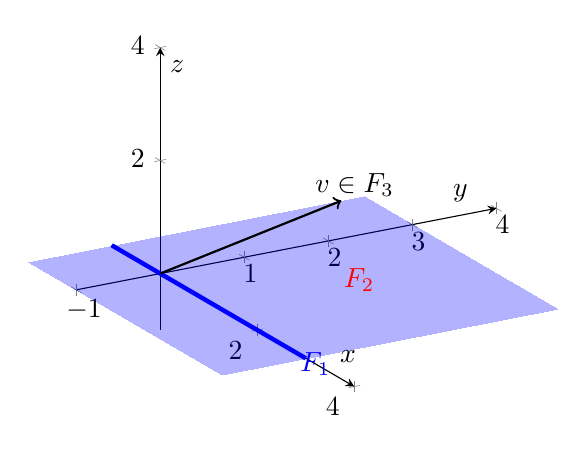
\begin{tikzpicture}
  \begin{axis}[
      view={60}{30},
      axis lines=center,
      xlabel={$x$},
      ylabel={$y$},
      zlabel={$z$},
      xmin=-1, xmax=4,
      ymin=-1, ymax=4,
      zmin=-1, zmax=4,
      samples=10,
      domain=-1:4,
      y domain=-1:4,
      z buffer=sort,
      width=10cm, height=8cm,
  ]
    % F1: Invariant line (x-axis)
    \addplot3[blue, ultra thick, domain=-1:3]({x},{0},{0});
    \node[blue] at (axis cs:3.2,0,0) {$F_1$};

    % \addplot3[->, black, thick] coordinates {(0, 0, 0) (2, 0, 0)};
    % \node[black, above] at (axis cs:2,0,0) {$v_1 = f(v_1)$};

    % F2: Invariant plane (xy-plane)
    \addplot3[
      surf,
      fill=red,
      opacity=0.3,
      shader=interp,
      samples=2,
      domain=-1:3,
      y domain=-1:3,
    ]
    ({x},{y},{0});
    \node[red] at (axis cs:1.5,1.5,0.2) {$F_2$};

    % Optionally: Draw a vector in F3 (illustrating the full space)
    \addplot3[black,->,thick] coordinates {(0,0,0) (2,1,2)};
    \node at (axis cs:2.1,1.1,2.3) {$v\in F_3$};

  \end{axis}
\end{tikzpicture}
\end{center}% --- CHUNK_METADATA_START ---
% needs_review: True
% src_checksum: 8cca275d57768137e37d787409628be302ecf03d302e568627928744fb85d595
% --- CHUNK_METADATA_END ---
Оскільки ми маємо інтуїтивне розуміння тригоналізовного ендоморфізму, повернімося до чистої математики.% --- CHUNK_METADATA_START ---
% needs_review: True
% src_checksum: a5db95e707fd8e6c77bc25fe420465e168c8220a57713ec7934ac000630976f2
% --- CHUNK_METADATA_END ---
\subsection{Теорія}% --- CHUNK_METADATA_START ---
% needs_review: True
% src_checksum: 36d1aae4a5b73157818018621c793b8b2714c671bc34e81fa36b07a1c002e80a
% --- CHUNK_METADATA_END ---
\begin{theorem}\label{thm:trigonalisable-si-scinde}
    Ендоморфізм є тригонализованим в $K$ тоді й тільки тоді, коли його характеристичний многочлен розкладається на лінійні множники в $K$.
    \par
    Це означає, що характеристичний многочлен має рівно $n$ коренів, де $n = \dim(E)$, і записується так:
     \[
         P_f(X) = (-1)^n(X - \lambda_1)^{\alpha_1}\cdots(X - \lambda_p)^{\alpha_p}
    \]
    де $\alpha_1 + \ldots + \alpha_p = n$
\end{theorem}% --- CHUNK_METADATA_START ---
% needs_review: True
% src_checksum: f27effc0e9df354b6ed9cf4b3da8028d3743bdcc47f10cfccbc3f5af24a25ec6
% --- CHUNK_METADATA_END ---
\begin{preuve} -
   \begin{itemize}
       \item[($\implies$)] Припустимо, ендоморфізм $f$ тригонізується, і нехай буде базис $\{e_1, \ldots, e_n\}$ такий що
           \[
               M(f)_{e_i} = \begin{pmatrix} 
                   a_{1,1} &            & & *\\
                   0       & a_{2, 2}   & & \\
                   \vdots  &      & \ddots & \\
                   0        & \ldots    & 0 & a_{n, n}
               \end{pmatrix} 
           \] 
           Маємо:
           \[
            P_f(X) = \det \begin{pmatrix} 
                   a_{1,1} - X &            & & *\\
                   0       & a_{2, 2} - X   & & \\
                   \vdots  &      & \ddots & \\
                   0        & \ldots    & 0 & a_{n, n} - X
               \end{pmatrix} = (a_{1,1} - X) \cdots (a_{n,n} - X)
           \] 
           Отже, $P_f(X)$ добре розщеплюється (можна помітити, що його корені — це власні значення $f$).
       \item[($\impliedby$)] Припустимо, $P_f(X)$ розщеплюється, і доведемо за індукцією, що $f$ тригонізується.
            \par
            Для $n=1$ тривіально.
            \par
            Припустимо, що результат вірний для порядку $n-1$. Але $P_f(X)$ розщеплюється, він має принаймні один корінь $\lambda_1 \in K$ і отже власний вектор $\varepsilon_1 \in E_{\lambda_1}$. Доповнимо $\{\varepsilon_1\}$ до базису $\{\varepsilon_1, \ldots, \varepsilon_n\}$, отже маємо:
            \[
            A = M(f)_{\varepsilon_i} = \begin{pmatrix} 
                \lambda_1 & b_2 & \ldots & b_n\\
                0         &     &        &    \\
                \vdots    &     & B      &    \\
                0         &     &        &
            \end{pmatrix}, \quad \text{де:} B \in \mathcal{M}_{n-1}(K)
            \] 
            Нехай $F = \operatorname{Vect}(\varepsilon_2, \ldots, \varepsilon_n)$ і $g: F \to F$ єдиний ендоморфізм $F$ такий що $M(g)_{\varepsilon_2, \ldots, \varepsilon_n} = B$, маємо:
            \[
            P_f(X) = \det(A - XI_n) = (\lambda_1 - X)\det(B - XI_{n-1}) = (\lambda_1 - X)P_g(X)
            \] 
            Але $P_f(X)$ розщеплюється, $P_g(X)$ також, і згідно з індуктивним припущенням $B$ тригонізується, отже існує базис $\{v_2, \ldots, v_n\}$ в якому $M(g)_{v_2, \ldots, v_n}$ є трикутною, і отже матриця $f$ у базисі $\{\varepsilon_1, v_2, \ldots, v_n\}$ є трикутною, отже $f$ тригонізується.
   \end{itemize} 
\end{preuve}% --- CHUNK_METADATA_START ---
% needs_review: True
% src_checksum: 9bb744e88dd97bc7d0ae2ea03d3215bcd3fccc78c15bc8f09bcfacaf14071d84
% --- CHUNK_METADATA_END ---
\begin{corollary}
    Будь-яка матриця $A \in \mathcal{M}_n(\mathbb{C})$  подібна до трикутної матриці з $\mathcal{M}_n(\mathbb{C})$.
\end{corollary}% --- CHUNK_METADATA_START ---
% needs_review: True
% src_checksum: a3b598c9377193bbd0acace6e3dff04e1b8fd3d50b29e18abeea54d26e5ab17c
% --- CHUNK_METADATA_END ---
\begin{intuition}
    Згідно з курсом абстрактної алгебри, кожен многочлен у $\mathbb{C}$ є розкладним. 
\end{intuition}% --- CHUNK_METADATA_START ---
% needs_review: True
% src_checksum: 23b673348e1d58c00e761620ff4fbfd71672707c2d007e5abd7f154f1199b206
% --- CHUNK_METADATA_END ---
\begin{remark}-
   \begin{enumerate}
       \item Якщо $A$ є тригонализовна і $A'$ трикутна, подібна до $A$, тому $A'$ має власні значення на діагоналях.
       \item Будь-яка матриця $A \in \mathcal{M}_n(K)$ є тригонализовна над замиканням $K'$ з $K$. (напр.: $A \in \mathcal{M}_n(\R)$ є тригонализовна над $\mathbb{C}$).
   \end{enumerate} 
\end{remark}% --- CHUNK_METADATA_START ---
% needs_review: True
% src_checksum: e9bf0c73c0a303936ab15442415a5c043bc85a10dfc78a9f1f25a77c3a1ef9ea
% --- CHUNK_METADATA_END ---
\begin{corollary}
    Нехай $A \in \mathcal{M}_n(K)$ і $\{\lambda_1, \ldots, \lambda_n\}$ її власні значення, тому
    \begin{align*}
        \operatorname{Tr}(A) = \lambda_1 + \ldots + \lambda_n\\
        \det(A) = \lambda_1 \cdot \ldots \cdot  \lambda_n
    \end{align*}
\end{corollary}% --- CHUNK_METADATA_START ---
% needs_review: True
% src_checksum: 6a64df61bb2708a9fd24ca53aed335fb8a45d67e1e7546c637a7189e188878fe
% --- CHUNK_METADATA_END ---
\begin{proof}
    Маємо $A' \in \mathcal{M}_n(K')$ трикутну, подібну до $A$ (нагадування: замикання $K'$ над $K$), отже власні значення знаходяться на діагоналях $A'$. Однак подібні матриці мають ті ж самі сліди та визначники, тому $\operatorname{Tr}(A) = \operatorname{Tr}(A') = \lambda_1 + \ldots + \lambda_n$ та $\det(A) = \det(A') = \lambda_1 \cdot \ldots \cdot \lambda_n$.
\end{proof}% --- CHUNK_METADATA_START ---
% needs_review: True
% src_checksum: 11b9712aef359491bca7e59c520beb8ba0147b020f46f80e8d4a24ca53be4c56
% --- CHUNK_METADATA_END ---
Ми покажемо процес тригоналізації на наступному прикладі:% --- CHUNK_METADATA_START ---
% needs_review: True
% src_checksum: 63a5151eafc8d99446d7ae80a68214a2a2a0a53070567819c88bf927fc0da0d7
% --- CHUNK_METADATA_END ---
\begin{eg}
   Нехай матриця 
   \[
   A = \begin{pmatrix}
       -4 & 0 & -2 \\
       0 & 1 & 0\\
       5 & 1 & 3
   \end{pmatrix}
   \] 
   Маємо характеристичний многочлен $P_A(X) = -(X - 1)^2(X + 2)$, який розщеплюється в $\R$, тому $A$ є тригоналізованою (згідно з теоремою \ref{thm:trigonalisable-si-scinde}), отже, якщо розглядати $A$ як ендоморфізм у канонічному базисі, ми знаємо, що існує базис  $\{v_i\}$ з  $\R^3$ такий що:
   \[
       M(f)_{v_i} = \begin{pmatrix} 
           1 & a & b\\
           0 & 1 & c\\
           0 & 0 & -2
       \end{pmatrix} 
   \] 
   я нагадую, що це означає:
   \begin{align}\label{eq:trigon-example-system}
       \begin{cases}
           f(v_1) = v_1\\
           f(v_2) = a v_1 + v_2\\
           f(v_3) = b v_1 + c v_2 - 2 v_3
       \end{cases}
    \end{align}

   Почнемо з пошуку $v_1$. Ми знаємо, що  $v_1$ є власним вектором, що відповідає власному значенню  $\lambda_1 = 1$, тобто  $(f - \operatorname{Id})v_1 = 0$, тому обчислимо $(A - I)v_1 = 0$ (іншими словами, ми шукаємо $v_1$, який породжує  $\ker(A - I)$) :
   \begin{align*}
       (A - I) \begin{pmatrix} x \\ y \\ z \end{pmatrix} \iff 
       \begin{cases}
           -5x    -2z & = 0\\
            5x  +y +2z &=0
       \end{cases}
    \end{align*}
    Тоді ми можемо взяти $v_1 = \begin{pmatrix} 2 \\ 0 \\ -5 \end{pmatrix} $ (іншими словами $\ker(A - I) = \operatorname{Vect}(\begin{pmatrix} 2 \\ 0 \\ -5 \end{pmatrix})$).

    Далі, шукаємо $v_2$, згідно з \ref{eq:trigon-example-system}, 
    \begin{align*}
        &f(v_2) = av_1 + v_2 \\
        \implies &f(v_2) - v_2 = av_1\\
        \implies &(f - I)v_2 = a v_1\\
        \implies &(A - I)v_2 = a v_1
    \end{align*}
    Отже, маємо:
    \[
        (A - I)\begin{pmatrix} x \\ y \\ z \end{pmatrix} = a \begin{pmatrix} 2 \\ 0 \\ -5 \end{pmatrix} \iff
        \begin{cases}
            -5x - 2z = 2a\\
            5x + y + 2z = -5a
        \end{cases}
    \] 
    Тоді, взявши $a = 1$, маємо 
    \[
        \begin{cases}
            -5x - 2z = 2\\
            5x + y + 2z = -5
        \end{cases}
    \] 
    тому $v_2 = \begin{pmatrix} -2 \\ -3 \\ 4 \end{pmatrix} $ (просто розв'язання системи).

    Для $v_3$ маємо два варіанти:
     \begin{enumerate}
        \item або діяти так само з розв'язанням системи
        \item або зауважити, що існує власний вектор $A$, що відповідає власному значенню  $-2$, тобто  $\exists v_3 \in \R^3$ такий що $f(v_3) = -2 v_3$, тоді ми можемо взяти цей вектор  $v_3$ і, отже, покласти  $b = c = 0$.
    \end{enumerate}
    \begin{remark}
       Чому ми можемо так робити? Тому що для кожного власного значення $f$ завжди існує власний простір кратності принаймні  $1$, отже, і для власного значення  $-2$ теж. 
    \end{remark}
    Тоді шукаємо $v_3$:
     \[
         (A + 2I)v_3 = 0 \iff \begin{cases}
             -2x - 2z = 0\\
             3y = 0
         \end{cases}
    \]
    тому ми можемо взяти $v_3 = \begin{pmatrix} 1 \\ 0 \\ -1 \end{pmatrix} $.
    
    Отже, матриця $A$ подібна до 
     \[
    A' = M(f)_{v_i} = \begin{pmatrix} 
        1 & 1 & 0\\
        0 & 1 & 0\\
        0 & 0 & -2
    \end{pmatrix} 
    \] 
    з матрицею переходу:
    \[
    P = \|v_1, v_2, v_3\| = \begin{pmatrix} 
        2 & -2 & 1\\
        0 & -3 & 0\\
        -5 & 4 & -1
    \end{pmatrix} 
    \] 
\end{eg}
